% REQUIRED: Declare the document class to be used.  Note: To format
% the dissertation signature page for online submission, comment the first
% ``documentclass'' line and uncomment the following line.
\documentclass{brandiss}
%\documentclass[online]{brandiss}

% Optional: The graphicx package eases inserting pictures in documents.
\usepackage{graphicx}

% Optional: the amssymb package includes many useful mathematical symbols.
\usepackage{amssymb}

% Optional: Number sections and figures within chapters.
\numberwithin{section}{chapter}
\numberwithin{figure}{chapter}

% REQUIRED: Dissertation information.  This information can be
% accessed with the \thediss{} command, as is shown in the document
% below.
\disstitle{Title}
\dissauthor{Sofiya Semenova}
\dissadvisor{Olga Papaemmanouil}
\dissdepartment{Computer Science}
\dissmonth{May}% My graduation month.
\dissyear{2017}% My graduation year.

% Optional: Define environments to ease creating definitions, theorems
% and remarks.  For proofs, use the ``proof'' environment.
\theoremstyle{definition}
\newtheorem{definition}{Definition} 
\theoremstyle{plain}
\newtheorem{theorem}{Theorem} 
\theoremstyle{remark}
\newtheorem{remark}{Remark} 

% Optional: Commands to make LaTeX equations use mathematical terms.
\newcommand{\into}{\hookrightarrow}
\newcommand{\onto}{\twoheadrightarrow}

\newcommand{\rC}{\mathbb C} % The field of complex numbers.
\newcommand{\pCP}{\mathbb{CP}} % The complex projective space.
\newcommand{\rZ}{\mathbb Z} % The ring of integers.
\newcommand{\mM}{\mathcal M} % A manifold M.

\DeclareMathOperator{\Homol}{H} % The co/homology functor.
\newcommand{\Partial}[2]{\dfrac {\partial #1} {\partial #2}}
\newcommand{\Hessian}[3]{\dfrac {\partial^2 #1} {\partial #2\partial #3}}

% The actual document begins.
\begin{document}

% REQUIRED: The start of roman-numbered plain pages.
\frontmatter

% REQUIRED: Create the dissertation title page.
\makedisstitle


\tableofcontents % REQUIRED

\listoffigures % optional

\listoftables % optional


% REQUIRED: The start of arabic-numbered fancy pages.
\mainmatter

\chapter{Introduction}

With the migration of database applications from enterprise-owned data centers to cloud environments, developers face many challenges with deploying data management applications on infrastructure as a service (IaaS) clouds. On the cloud, data processing services can be paid for individually and on-demand, so an ideal solution to workload management problems would minimize monetary constraints while supporting different performance goals.

Previously, this task would fall to database administrators, who would have to spend time to solve these problems on a case-by-case basis. Further, while simple versions of these problems are easy to solve, very complex examples are not intuitive to reason about and thus become difficult to solve. We would like to automate as much of this task for the DBA as possible. Machine learning offers a learning-based approach to solving these problems, freeing up DBA time, as well as coming up with better solutions. My thesis focuses on developing machine learning approaches to some of these workload management related problems.

One common problem is that of resource provisioning (the provisioning of new VMs), workload distribution (placing queries on VMs), and query scheduling (the order in which to run queries). WiSeDB and BanditDB are two different machine learning based approaches to this problem; WiSeDB uses supervised learning, whereas BanditDB uses reinforcement learning. While these two approaches already address this problem, the two systems were unified into a single workload management service for my thesis. 

Another problem is that of data-driven fragmentation and fragment distribution, which we address in the ongoing work. Data fragmentation is concerned with how split tables in a database into fragments, while fragment distribution is concerned with how many copies of each fragment to create, and which fragments to place on which VMs.

My senior thesis focused on unifying WiSeDB and BanditDB into a single prototype that would demonstrate each strategy, as well as to design and implement a solution to the problem of data fragmentation.

% Force a new page.
\clearpage

\chapter{WiSeDB}

Consider the following problem: in Figure~\ref{fig:wisedb-example1}, we are given four blocks - two with a size of 8 units, and two with a size of 2 units. We would like to pack these blocks in as few bins as possible. What is the optimal way to pack these blocks if no bin is larger than 8 units?

\begin{figure}[htbp]
  \centering
  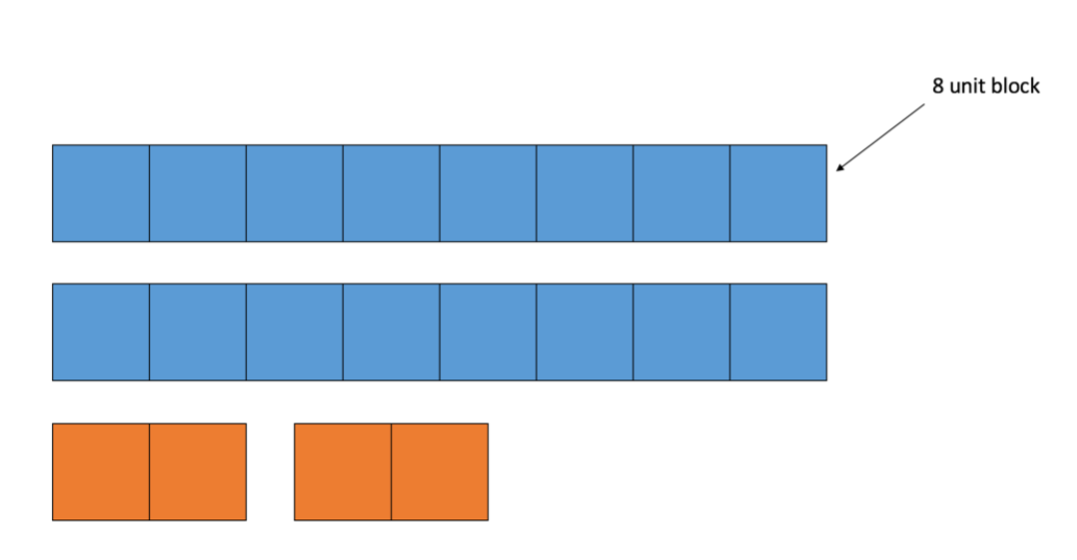
\includegraphics[height=2in]{wisedb-example1}
  \caption{An Example Workload}
  \label{fig:wisedb-example1}
\end{figure}

The optimal solution, as demonstrated in Figure~\ref{fig:wisedb-example2}, is to place the two 8-unit blocks into their own bins, and the two 2-unit blocks together into one bin. This packing is equivalent to first-fit-decreasing (FFD) - a common heuristic that places blocks in order of decreasing size.

What if the bins are no larger than 10 units? Figure~\ref{fig:wisedb-example3} demonstrates that we can get rid of an entire bin by pairing together an 8-unit block and a 2-unit block into each bin. If we were to use FFD for this example, we'd end up with Figure~\ref{fig:wisedb-example2} again - two bins with 8-unit blocks on their own, and another bin with two 2-unit blocks. We have enough space in our first to blocks to fit the 2-unit blocks, but using the FFD heuristic does not give us that optimal solution.

\begin{figure}[htbp]
  \centering
  \includegraphics[height=2in]{wisedb-example2}
  \caption{Optimal Solution with Bins of Size 8}
  \label{fig:wisedb-example2}
\end{figure}

\begin{figure}[htbp]
  \centering
  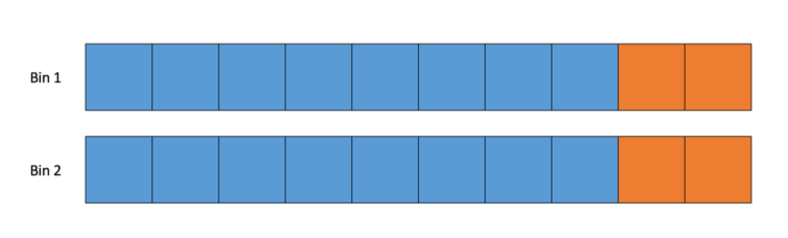
\includegraphics[height=1.5in]{wisedb-example3}
  \caption{Optimal Solution with Bins of Size 10}
  \label{fig:wisedb-example3}
\end{figure}

This example mirrors the problems of research provisioning, query placement, and query scheduling. The blocks are queries, the units are the amount of time it takes each query to complete (the latency), the bins are VMs, and the bin size is the amount of time we want all the queries to be completed within (the SLA). The result - a list of bins with blocks in them - is the workload schedule.

This example is simple, but reasoning about the optimal solution becomes more difficult as workload specifications get more complex. To that end, we want to automate as much of this task for the DBA as possible. Using machine learning techniques, our goal is to generate a cost-effective workload schedule based on specific workload characteristics and performance goals while minimizing the cost of using cloud resources. 

WiseDB is a batch-scheduling approach to this problem. It uses supervised learning on a random training set to generate decision trees, which are used to schedule a batch of queries.


\section{Previous Research}

Previous solutions have addressed each of the three problems in isolation, which leads to difficulty in integrating the three separate systems and configuring them to work together. Further, while the systems the solutions are designed for require a wide range of performance metrics, previous solutions have not incorporated many different types of performance metrics into their approaches.

\section{WiSeDB Approach}

Using a workload specification and performance metrics provided by the user, WiseDB generates a decision tree based on a similar sample workload. In this decision tree, the nodes are features - characteristics about the provisioned VMs and workload specification. Using the decision tree, WiseDB schedules queries and provisions VMs one-by-one, based on a workload that the user inputs.

The performance metrics are input as Service Level Agreements (SLA). An SLA is a guarantee that the service provider will process all queries within a certain amount of time. In return for processing the query within that time frame, the user pays the service provider a cost, which takes into account the strictness of the SLA, the cost of provisioning VMs, and the penalty function for missing a deadline. Each generated model is designed to minimize the cost the user pays to the provider while meeting application defined performance goals. An SLA is input as a value and a type, where the type can be:

\begin{enumerate}
\item \textbf{Max} - all queries will be completed within X amount of time
\item \textbf{Per Query} - each query will take no longer than X time to complete
\item \textbf{Percentile} - 90\% of queries will be completed within X amount of time
\item \textbf{Average} - the average time it takes to complete a query is X
\end{enumerate}

WiseDB is designed to handle efficient scheduling of a batch workload, where the templates/query types of the workload are known a priori. This implies that we also have a way to predict or know in advance the expected execution time of each incoming query (also known as the latency).

******The WiSeDB approach *******

\section{Generating the Decision Tree}

To generate the decision tree, a user first must submit a workload specification and performance metrics. A workload specification takes the form of a list of query templates, while performance metrics  are input as an SLA amount and type. Based on the workload specification, WiSeDB generates sample workloads. Then, for each sample workload, an optimal schedule is generated by:

\begin{enumerate}
\item Represent scheduling decisions as edges with a weight equal to the cost of performing that decision
\item Find a minimum path through the graph

\end{enumerate}

Once the optimal schedule is generated for each sample workload, a training set is generated for the decision tree classifier. The training set contains pairs of decisions and the features that were present when that decision was made. The features are then extracted to form a decision tree.

***EXAMPLE OF GOING THROUGH THE TREE***

\begin{figure}[htbp]
  \centering
  \includegraphics[height=2in]{dt1}
  \caption{A Sample Decision Tree}
  \label{fig:dt1}
\end{figure}

\chapter{BanditDB}

Like WiSeDB, BanditDB is a machine learning based approach to the problems of resource provisioning, workload distribution, and query scheduling. However, unlike WiSeDB, BanditDB approaches this problem using reinforcement learning instead of supervised learning.

For WiseDB, a batch schedule is generated after the input of a workload specification and performance model. The latency - the amount of time it takes a query to run - is a necessary part of the workload specification. However, latency is difficult to measure and often not accurate, so it would be preferable to remove the dependency on that. A solution to end the reliance on latency predictions is to actually run the query and record how long it takes.

Further, because WiseDB is a batch scheduler, it does not take into account how workloads may change over time - there may be a lot of similar queries sent on the weekend, and an entirely different set of queries sent on weekdays. WiseDB's schedule might only work well for one of them. We can add the ability for the schedule to adapt to changes in the workload specification and resource availability by building a system that can learn from its decisions and adapt its future actions accordingly.

Thus, an improved approach would be to continually send new queries to the system, placing them on VMs by some common heuristic at first, until enough information is learned about the system. After each decision to place a query on a VM, the performance of that query is evaluated and used to make better decisions in the future. This solution is an example of reinforcement learning, which solves the problem well because it learns by evaluating actions and the results of those actions, rather than requiring a lot of information the DBA may not necessarily know.

\section{BanditDB Approach}

The reinforcement learning process contains three factors: a context, a decision, and an observation. The context includes the characteristics (features) of the system, the decision is a scheduling decision about the query, and the observation includes the results of the decision. To understand the reinforcement learning process, one useful reinforcement learning abstraction is contextual multi-armed bandits.

A gambler plays on a row of slot machines - called one-armed bandits - and needs to decide which slot machine arms to pull to maximize the sum of rewards received. For each round, the gambler decides a bandit to play, pulls the arm, and observes the result of the action - the amount of money they win or lose. By continually pulling arms on different bandits, the gambler can use the information they gained from their past experiences to come up with a strategy.

BanditDB uses a tiered system of contextual multi-armed bandits. These multi-armed bandits are arranged into tiers where each tier has 1 or more bandit (see Figure~\ref{fig:bandit}). In this case, the bandits are VMs and the tiers represent different types of VMs offered by the service provider.

\begin{figure}[htbp]
  \centering
  \includegraphics[height=2in]{bandit}
  \caption{Tiers of Multi-Armed Bandits}
  \label{fig:bandit}
\end{figure}

As queries arrive one-by-one, they enter the system to be placed. To place a query, BanditDB starts at the first VM in the highest tier and is allowed to make any of the following decisions:

\begin{enumerate}
\item \textbf{Accept} - place the query at the current VM
\item \textbf{Down} - move the query to the next tier. If there isn't a VM on that tier, create one
\item \textbf{Pass} - move the query to the next VM on the same tier. If there isn't a VM to go to, create one
\end{enumerate}

After making a decision (Accept, Down, or Pass), the system takes note of the features in the context that were available at the time of the decision. These features are characteristics about the current state of the system. Based on the context, the decision, and the results of that decision, the system improves upon its future decisions.

While there are many different types of characteristics that could be captured, we don't want to store them all because it would take the system too long to learn. However, we want to store enough to accurately describe the current state. Some features that are used are:

\begin{enumerate}
\item Tables in the database that the query uses
\item Memory availability
\item Number of queries in the queue
\item I/O rate
\item Network cost
\end{enumerate}

\chapter{Demo}

In the demo I created for my thesis, I combined the WiSeDB and BanditDB systems into one demo application. This application allows the user to specify their workload specification as sample query templates and their performance metrics as an SLA and SLA type. Then, they are able to select between the supervised learning approach (WiSeDB) and the reinforcement learning approach (BanditDB). Figure~\ref{fig:demo-screenshot} shows the user input section of the demo, Figure~\ref{fig:demo-supervised} shows the WiSeDB results, and Figure~\ref{fig:demo-reinforcement} shows the BanditDB results.

\begin{figure}[htbp]
  \centering
  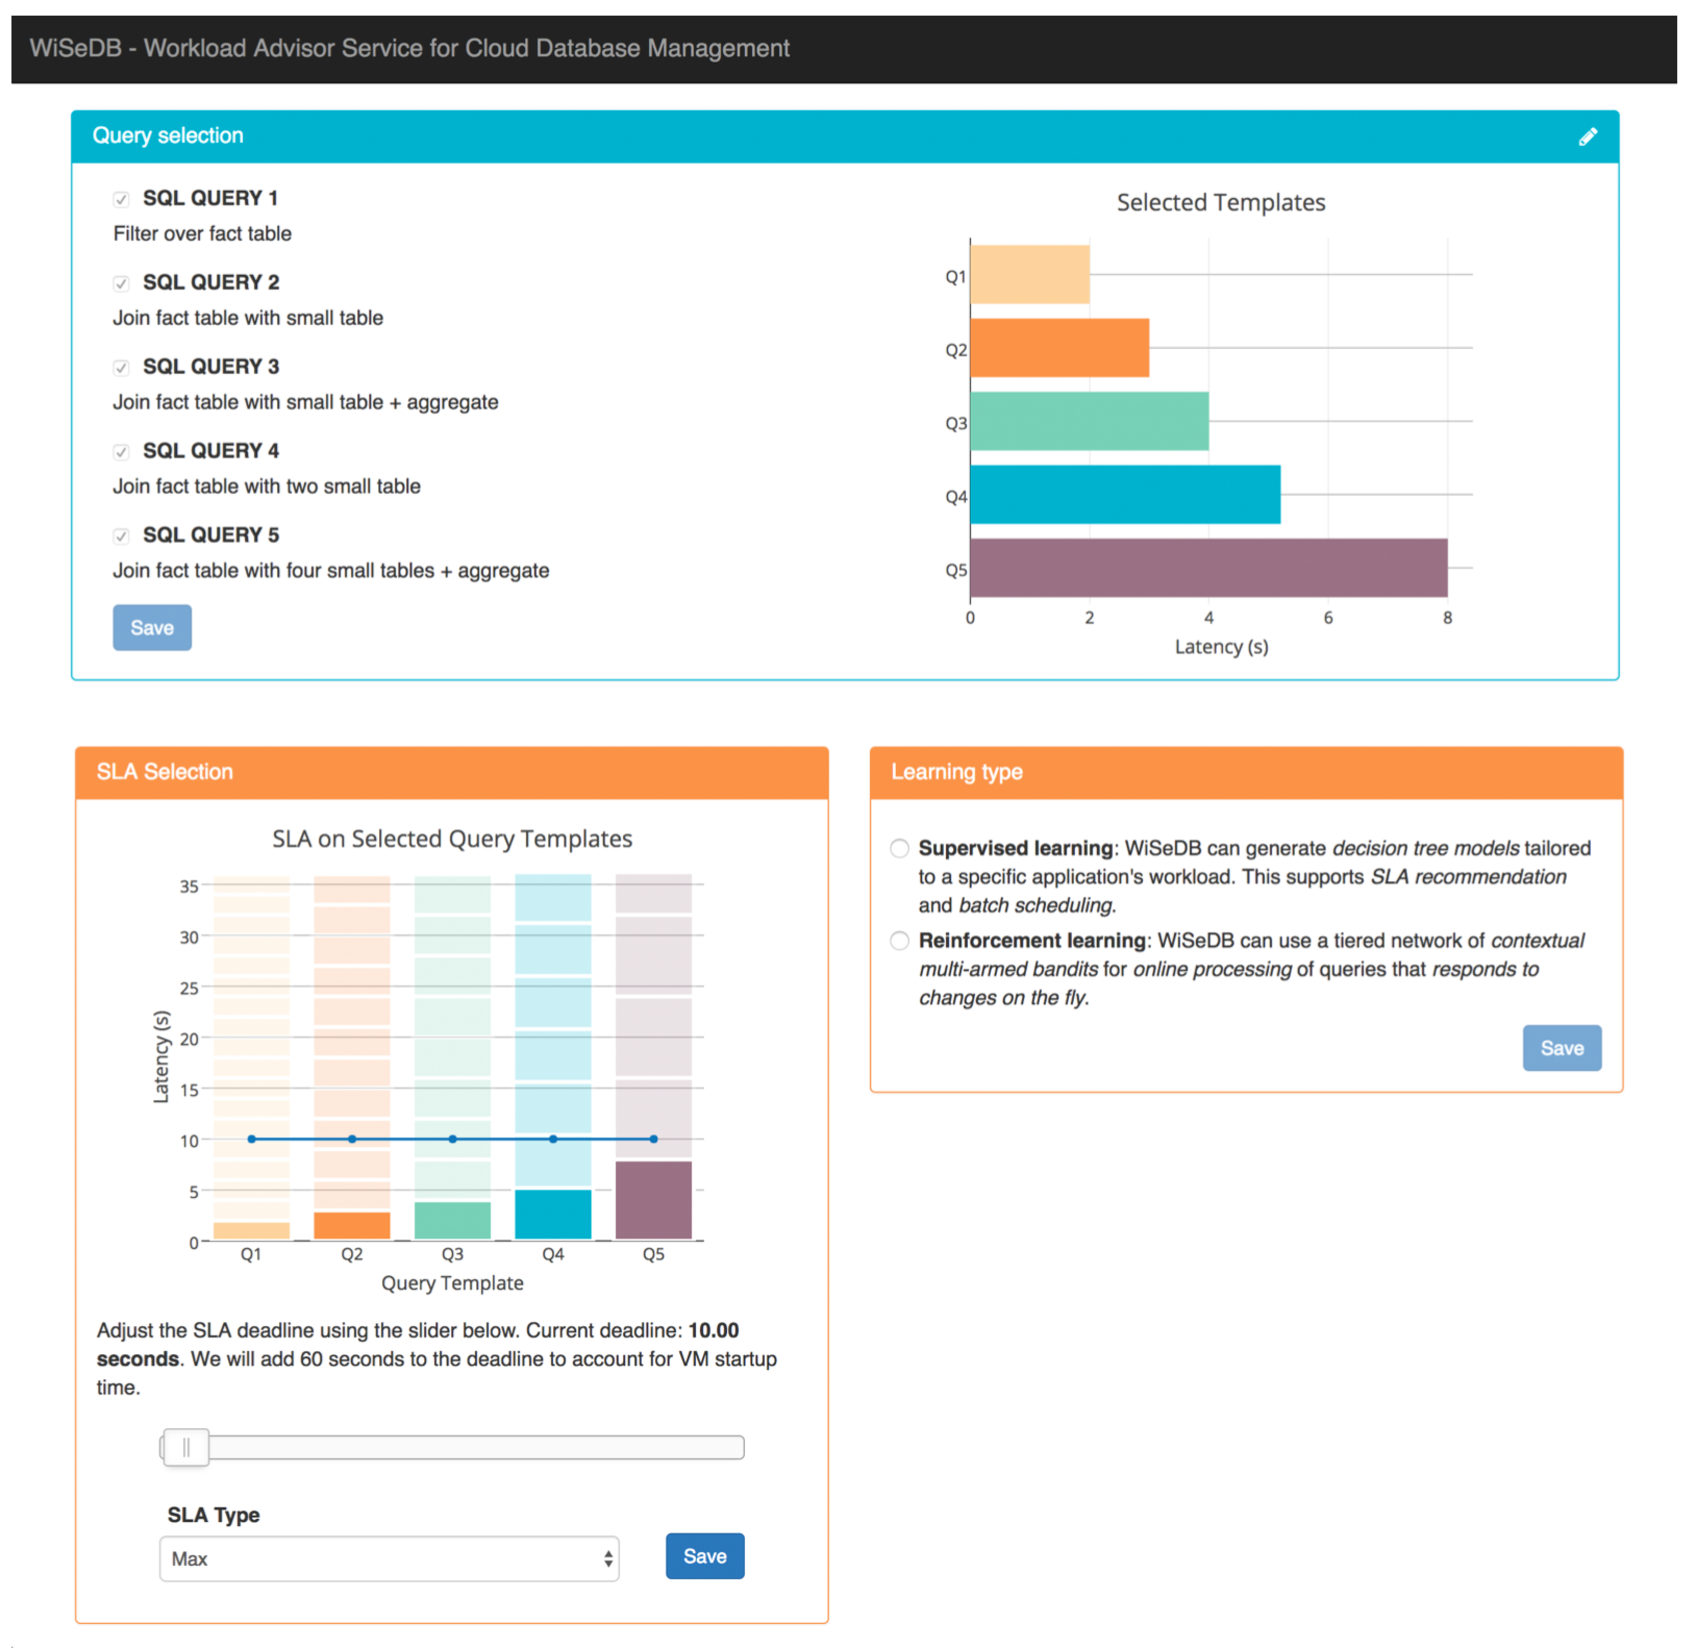
\includegraphics[height=5in]{demo-screenshot}
  \caption{User Input Section of Demo}
  \label{fig:demo-screenshot}
\end{figure}

\begin{figure}[htbp]
  \centering
  \includegraphics[height=5.5in]{demo-supervised}
  \caption{Results with Supervised Learning Selected}
  \label{fig:demo-supervised}
\end{figure}

\begin{figure}[htbp]
  \centering
  \includegraphics[height=5in]{demo-reinforcement}
  \caption{Results with Reinforcement Learning Selected}
  \label{fig:demo-reinforcement}
\end{figure}

\chapter{Ongoing Work}

With IaaS clouds, a database is split up into sections (fragments) and distributed across multiple VMs in a network. When a query arrives, it arrives at a particular VM, which has to either: process the query if it has all the data it needs locally stored, or request the data from another node(s).

Requesting data from another node takes time (communication cost), and might make it harder for a query to be completed within a performance metric. To minimize that, it would make sense to store all the fragments on each VM, but each VM has limited space and it is redundant to have so many copies of the database.

We want to figure out where to split up the database into fragments, how many copies of each fragment to have, and where to place those copies. We approach this problem with a profit-based model, where each VM seeks to maximize its profit and the system seeks to minimize the amount of VMs used, given that each VM has a space constraint. Our approach keeps track of how often the tuples in each fragment are accessed by different queries and uses that information to distribute fragments, split fragments into two, and join fragments together. 

\section{Previous Research}

There are two previous systems that we researched - Mariposa and SWORD.

In Mariposa, a centrally-planned economy is responsible for much of the decision-making. In the economic system, nodes bid for queries in auctions and a broker decides on winning nodes. Additionally, nodes can buy fragments from other nodes, sell fragments to other nodes, and delete their fragments. With a system based on monetary transactions, nodes would always seek to minimize their expenses and maximize their profits.

With Mariposa, a problem arises around the broker: a centrally-planned economy with a broker controlling all transactions introduces a lot of overhead and could be simplified with a more distributed system of decision-making. Furthermore, Mariposa relies on monetarily quantifying transactions between nodes, the broker, and the user, but the money used in the Mariposa system does not translate to real money. This creates a barrier for the user to interact with the system. Lastly, Mariposa includes a lot of confusing and lengthy implementation details, such as update streams and different types of advertisements, that make it difficult to implement and use.

SWORD includes a hypergraph-based approach to database fragmentation. The system first creates a hypergraph where the nodes are rows in a database and edges are queries. Then, SWORD minifies the hypergraph by combining similar rows and queries, and finds the optimal cut of the minimal graph. While this approach has good results, a lot of overhead and computational time is needed to create the hypergraph, minify it, and find the optimal cut. This process gets significantly more time-intensive as the amount of queries increases.

\section{Our Research}

Our research focuses on a solution to the problems of making fragments and assigning fragments to VMs by using a real-world money model to minimize the amount of provisioned VMs. Same-size fragments are initially created using value-based fragmentation, duplicated based on how frequently they are accessed, and then distributed across VMs according to the following properties:

\begin{enumerate}
\item Minimize the amount of VMs needed
\item Two or more fragments of the same type may not appear on the same VM
\end{enumerate}

This type of bin-packing is called class-constrained bin-packing.

After each "round" of query processing, the variance of fragments is calculated, and a random fragment is chosen to be split or joined. For a given fragment, we compute the expected income per share (copy) and the cost of storing a fragment on the machine. We create enough shares that the profit approaches, but doesn't go below, 0. The fragments are then re-distributed among the VMs. Our approach guarantees a nash equilibrium because, after re-distribution, no VM can gain more profit by obtaining another fragment.

\section{Splitting and Joining Fragments}

After each round, the variance of each fragment is computed based on the density estimate of its tuples. The density estimate corresponds to the average dollar value of a tuple, which correlates to how often the tuple was accessed by queries in the past. A high variance means that some tuples in a fragment were accessed far more often than other tuples, whereas a low variance means that all the tuples in a fragment were accessed about the same amount of times.

If a fragment with high variance were to be replicated, the lower-accessed tuples would be over-replicated, as it isn't necessary to make so many copies of them, and the higher-accessed tuples would be under-replicated, so there wouldn't be \textit{enough} copies made of them.

After the variance for each fragment has been found, a fragment is chosen based on a weighted random choice. This fragment is then split into two fragments by finding the optimal split point, which is defined as the point where, had the fragment been split, the two resulting fragments would each have the lowest variance possible.

Then, for each group of three consecutive fragments, the variance of each fragment individually is compared to the variance had the three fragments been joined into two. They are joined if it would result in a decrease of variances across the board.

Joining fragments, though it may appear to initially be counterintuitive, is advantageous because there is a minimum fragment size. If fragments can never be joined, optimal splits may not be found.

% REQUIRED: The start of arabic-numbered plain pages.
% GSAS formatting allowance: The back may be single-spaced.
\backmatter
\singlespacing
\bibliographystyle{amsplain}% Bibliography.
\bibliography{topology}

\end{document}

